  \subsection{Análisis de una forma de onda cuadrada}
    Se propone realizar el análisis en frecuencia de una señal de forma cuadrada, recordando que
    su espectro posee, de forma ideal, infinitos armónicos impares. Lo primero que se realiza es 
    la calibración de las puntas del osciloscopio.

    Luego, se conecta el generador al osciloscopio configurado con una \textbf{onda cuadrada} de
    frecuencia $\mathbf{f=1~kHz}$, y amplitud arbitraria. El menú del canal 1 se configura de la
    siguiente manera: \textbf{Acoplamiento CC}, \textbf{Sin límite de ancho de banda},
    \textbf{Sonda x10} y \textbf{No invertido}. Luego, para poder observar el espectro se
    se configura el menú matemático como sigue: \textbf{FFT}, \textbf{CH1}, \textbf{Rectangular},
    y \textbf{Zoom x1}. La Figura~\ref{fig:SeñalCuad1k} muestra esta señal en tiempo y frecuencia.

    \begin{figure}[H]
      \centering
      \begin{subfigure}[H]{0.42\textwidth}
        \frame{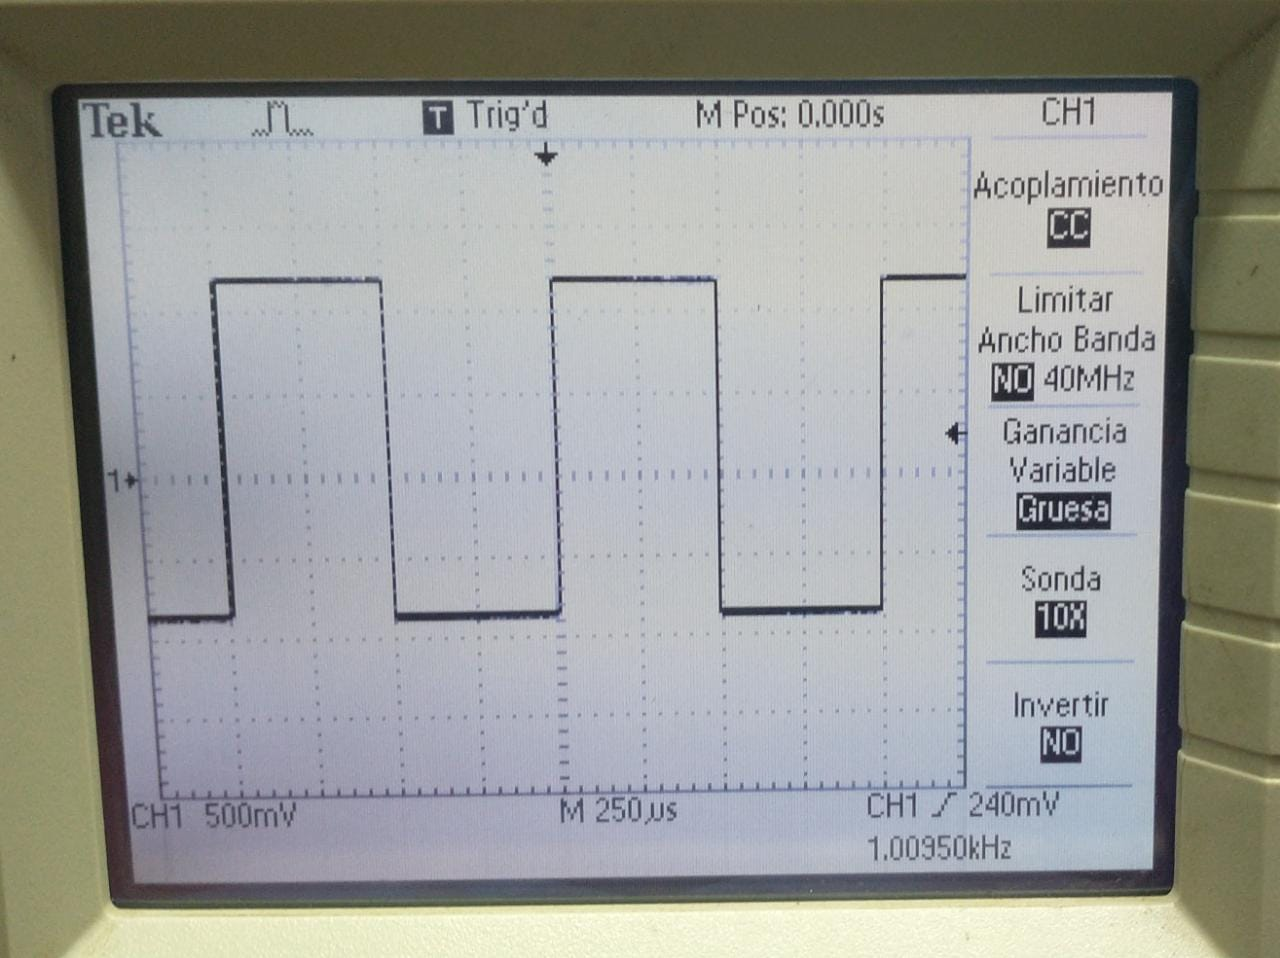
\includegraphics[width=\textwidth]{Imagenes/ActividadPractica/1AnalisisDeUnaSeñalCuadrada/Exp1_SeñalCuadrada1k_tiempo.jpeg}}
        \caption{En tiempo.}
      \end{subfigure}
      \hfill 
      \begin{subfigure}[H]{0.44\textwidth}
        \frame{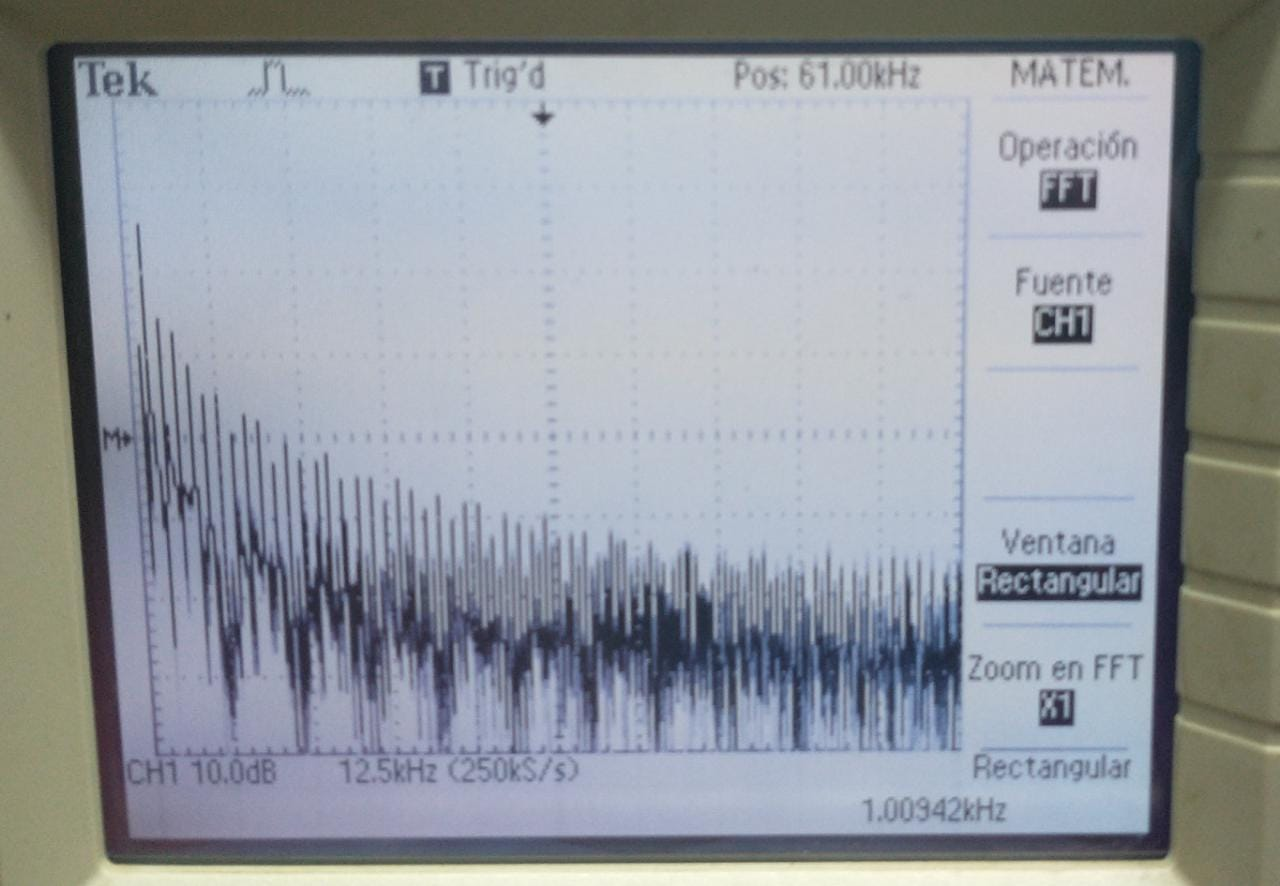
\includegraphics[width=\textwidth]{Imagenes/ActividadPractica/1AnalisisDeUnaSeñalCuadrada/Exp1_SeñalCuadrada1k_frec.jpeg}}
        \caption{En frecuencia.}
      \end{subfigure}

      \caption{Señal cuadrada de $1~kHz$.}
      \label{fig:SeñalCuad1k}
    \end{figure}

    A continuación, se procede a analizar los tipos de \textbf{adquisión} y \textbf{ventanas} con la misma señal
    previamente configurada. Para ello, se elige la opción \textbf{Zoom x10}. En la Figura~\ref{fig:SeñalCuadModoNormal}
    se muestran las distintas ventanas para el modo de adquisición \textbf{normal}.

    \begin{figure}[H]
      \centering
      \begin{subfigure}[H]{0.40\textwidth}
        \frame{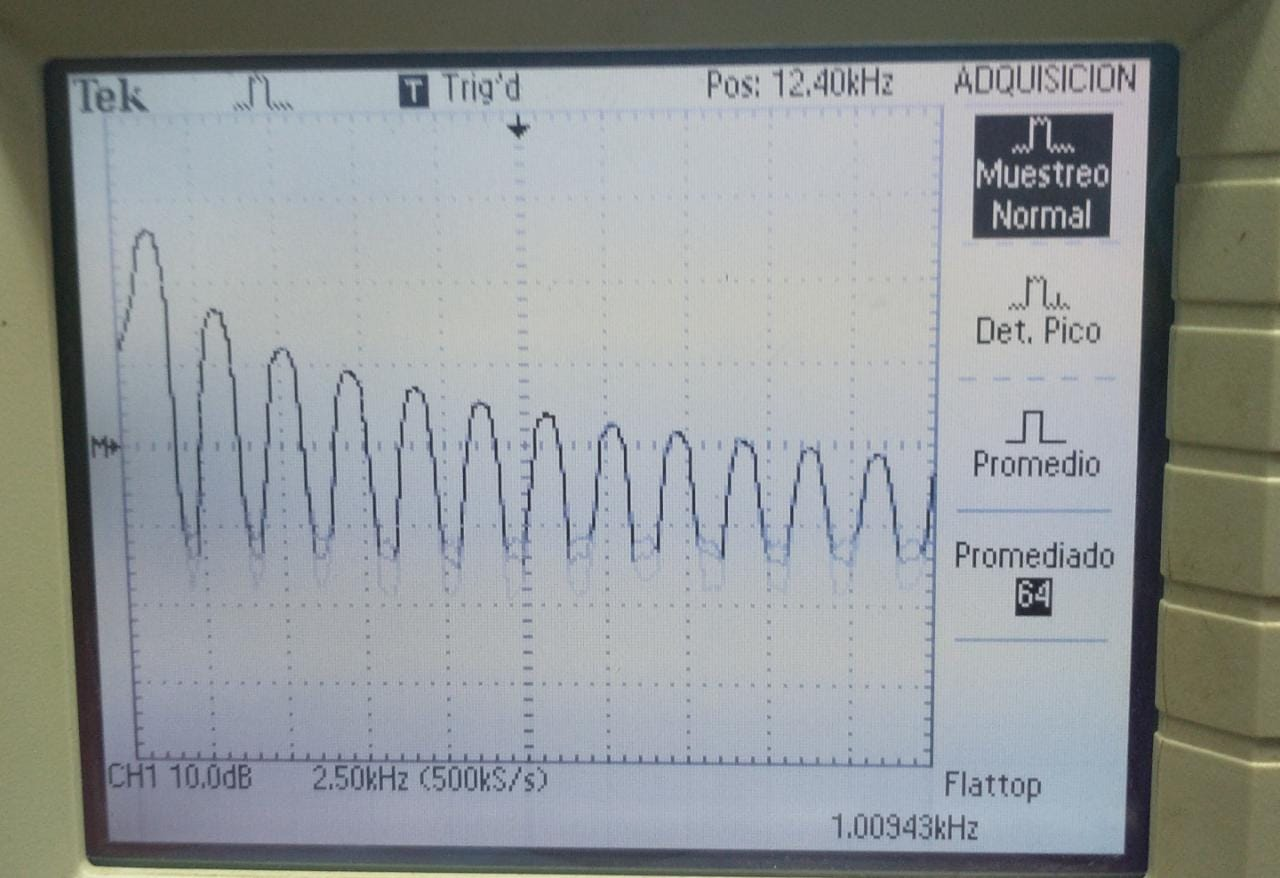
\includegraphics[width=\textwidth]{Imagenes/ActividadPractica/1AnalisisDeUnaSeñalCuadrada/Exp1_SeñalCuadrada_Normal_Flattop.jpeg}}
        \caption{Con ventana Flattop.}
      \end{subfigure}
      \hfill 
      \begin{subfigure}[H]{0.39\textwidth}
        \frame{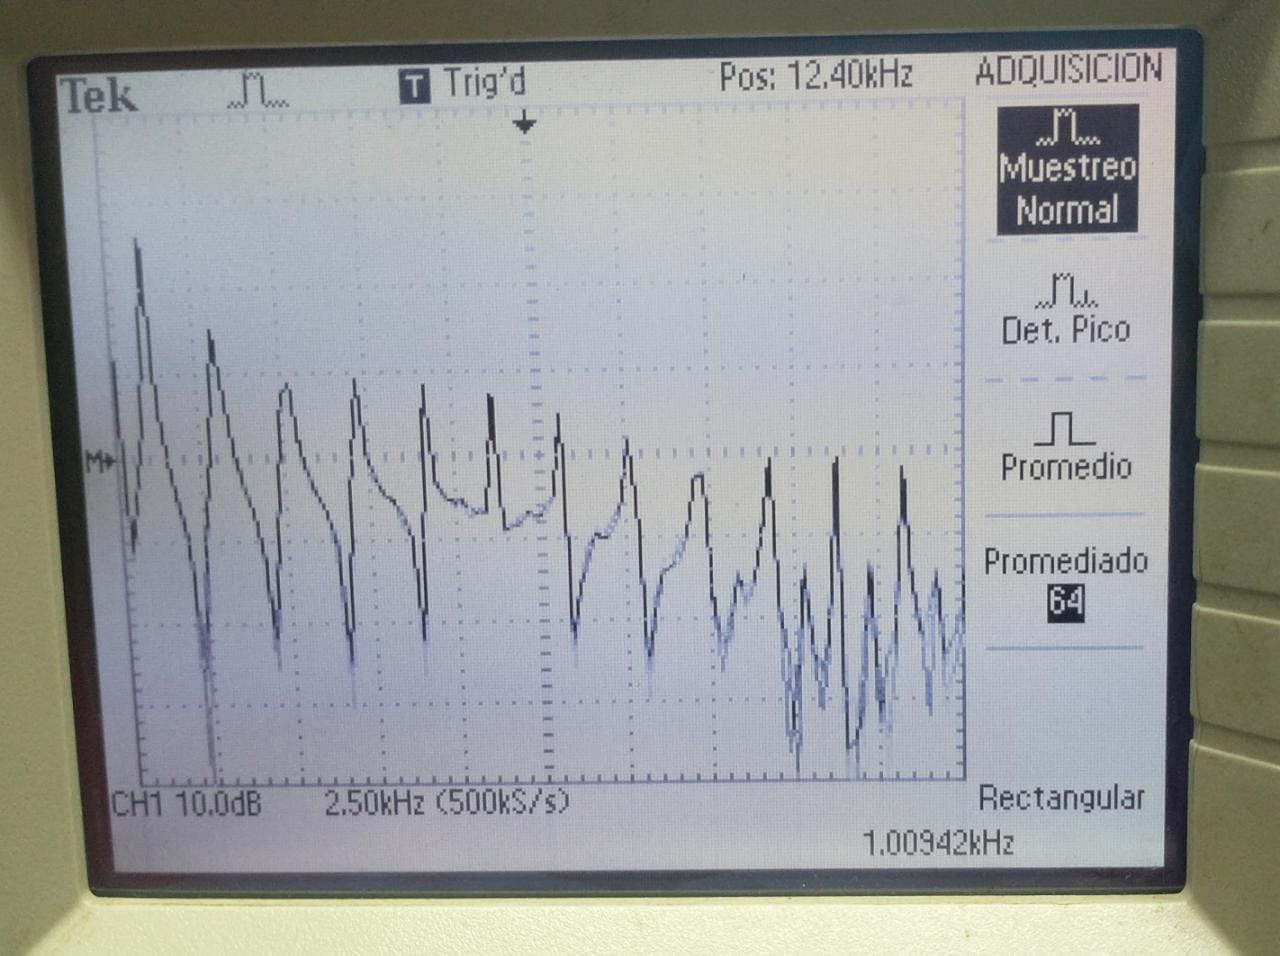
\includegraphics[width=\textwidth]{Imagenes/ActividadPractica/1AnalisisDeUnaSeñalCuadrada/Exp1_SeñalCuadrada_Normal_Rectangular.jpeg}}
        \caption{Con ventana Rectangular.}
      \end{subfigure}
      \hfill 
      \begin{subfigure}[H]{0.40\textwidth}
        \frame{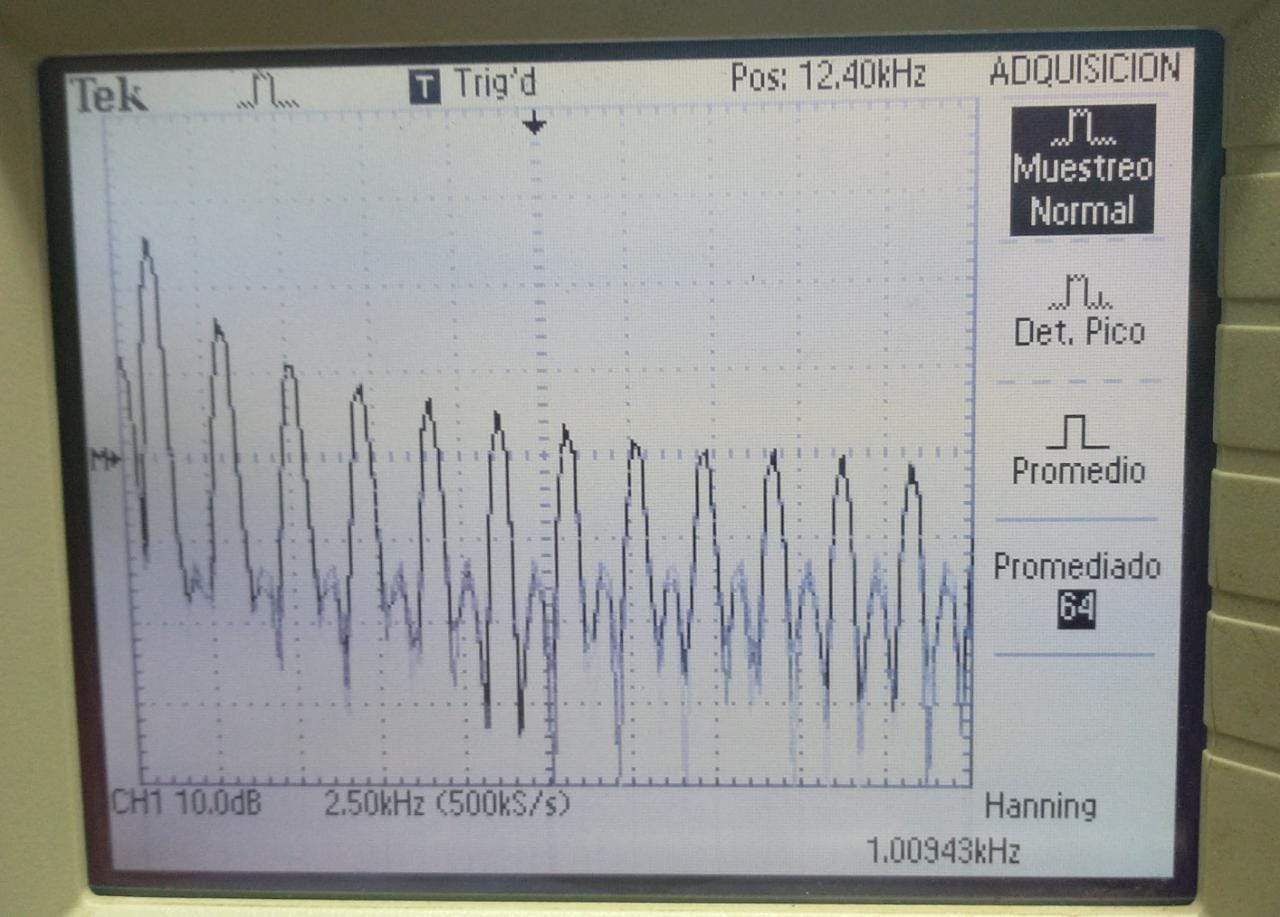
\includegraphics[width=\textwidth]{Imagenes/ActividadPractica/1AnalisisDeUnaSeñalCuadrada/Exp1_SeñalCuadrada_Normal_Hanning.jpeg}}
        \caption{Con ventana de Hanning.}
      \end{subfigure}

      \caption{Señal cuadrada de $1~kHz$ con modo de adquisición normal..}
      \label{fig:SeñalCuadModoNormal}
    \end{figure}

    Ahora, se selecciona el modo de adquisición de \textbf{detección de picos} y se varían los tipos de ventanas.
    Esto se encuentra en la Figura~\ref{fig:SeñalCuadModoDetecPicos}.
    \begin{figure}[H]
      \centering
      \begin{subfigure}[H]{0.40\textwidth}
        \frame{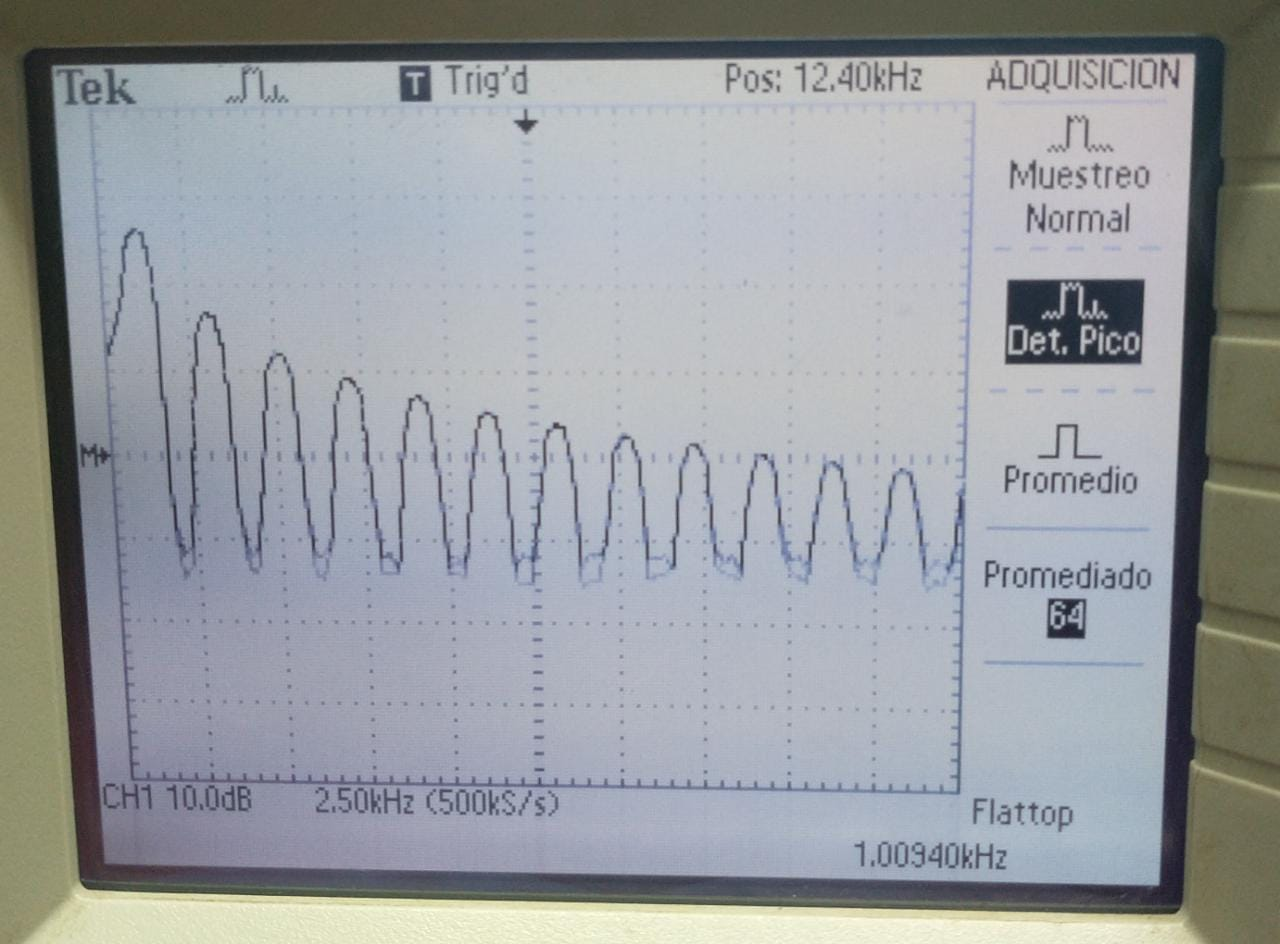
\includegraphics[width=\textwidth]{Imagenes/ActividadPractica/1AnalisisDeUnaSeñalCuadrada/Exp1_SeñalCuadrada_DecPicos_Flattop.jpeg}}
        \caption{Con ventana Flattop.}
      \end{subfigure}
      \hfill 
      \begin{subfigure}[H]{0.40\textwidth}
        \frame{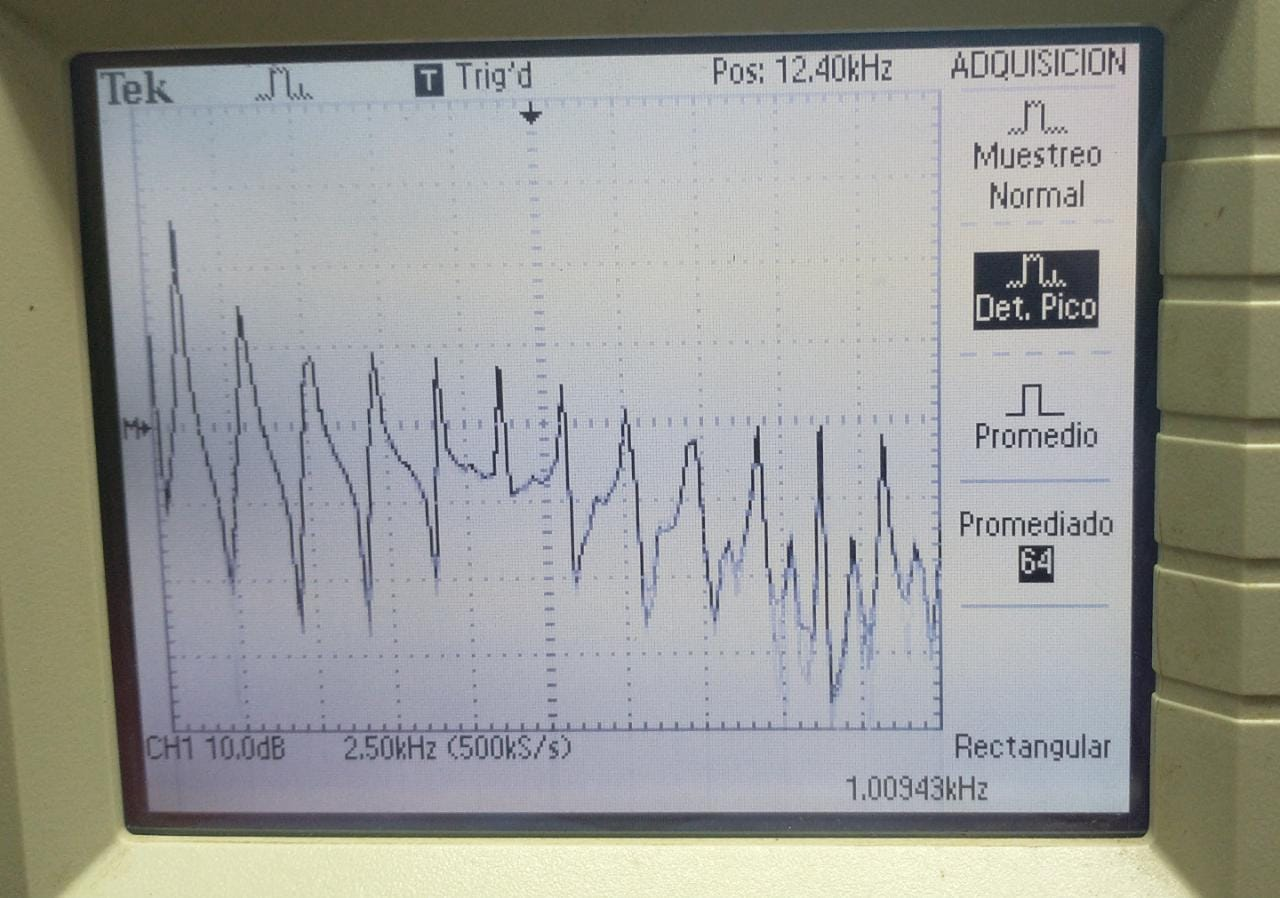
\includegraphics[width=\textwidth]{Imagenes/ActividadPractica/1AnalisisDeUnaSeñalCuadrada/Exp1_SeñalCuadrada_DecPicos_Rectangular.jpeg}}
        \caption{Con ventana Rectangular.}
      \end{subfigure}
      \hfill 
      \begin{subfigure}[H]{0.40\textwidth}
        \frame{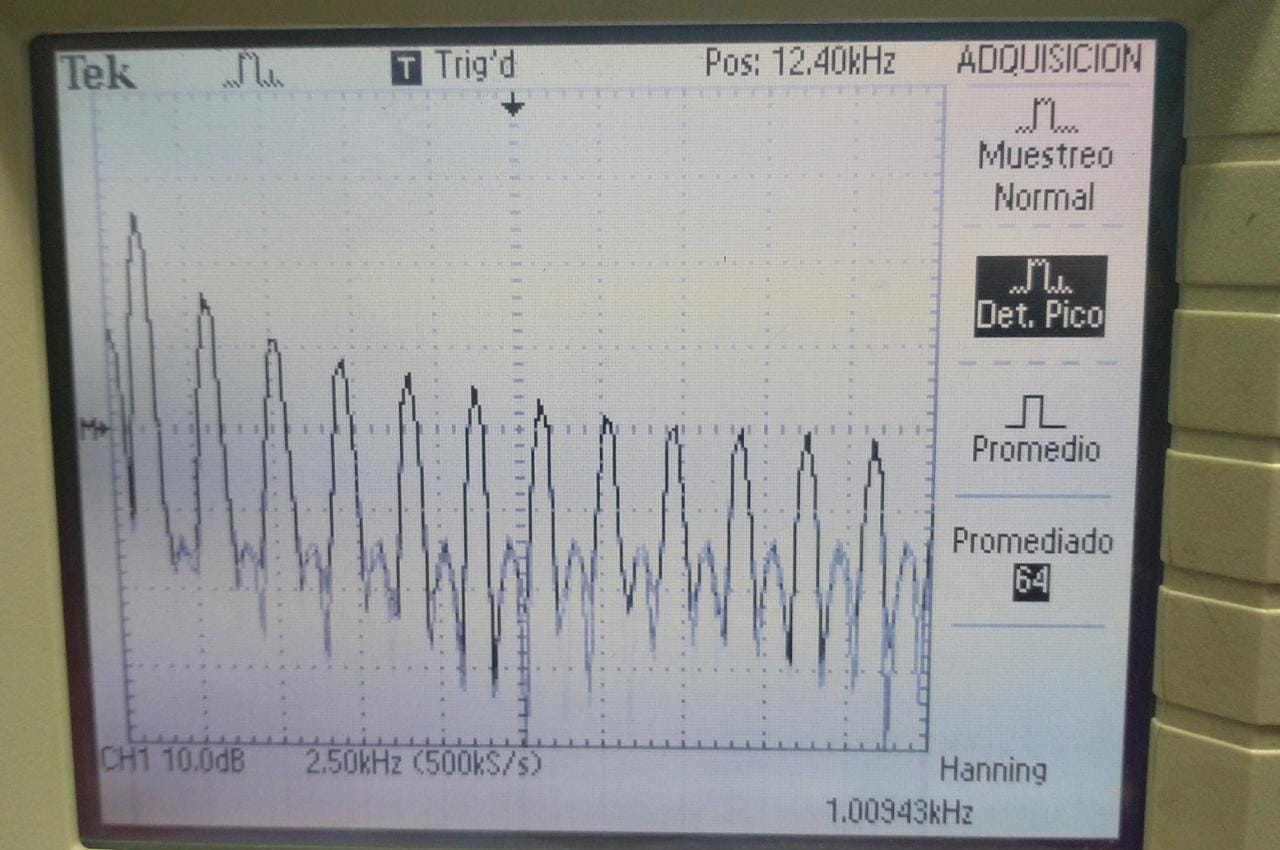
\includegraphics[width=\textwidth]{Imagenes/ActividadPractica/1AnalisisDeUnaSeñalCuadrada/Exp1_SeñalCuadrada_DecPicos_Hanning.jpeg}}
        \caption{Con ventana de Hanning.}
      \end{subfigure}

      \caption{Señal cuadrada de $1~kHz$ con modo de adquisición de detección de picos.}
      \label{fig:SeñalCuadModoDetecPicos}
    \end{figure}

    Finalmente, se pone a prueba el modo de adquisición \textbf{promedios}, para el cual se eligen
    \textbf{64 cuentas}. Esto se encuentra en la Figura~\ref{fig:SeñalCuadModoPromedio}.

    \begin{figure}[H]
      \centering
      \begin{subfigure}[H]{0.40\textwidth}
        \frame{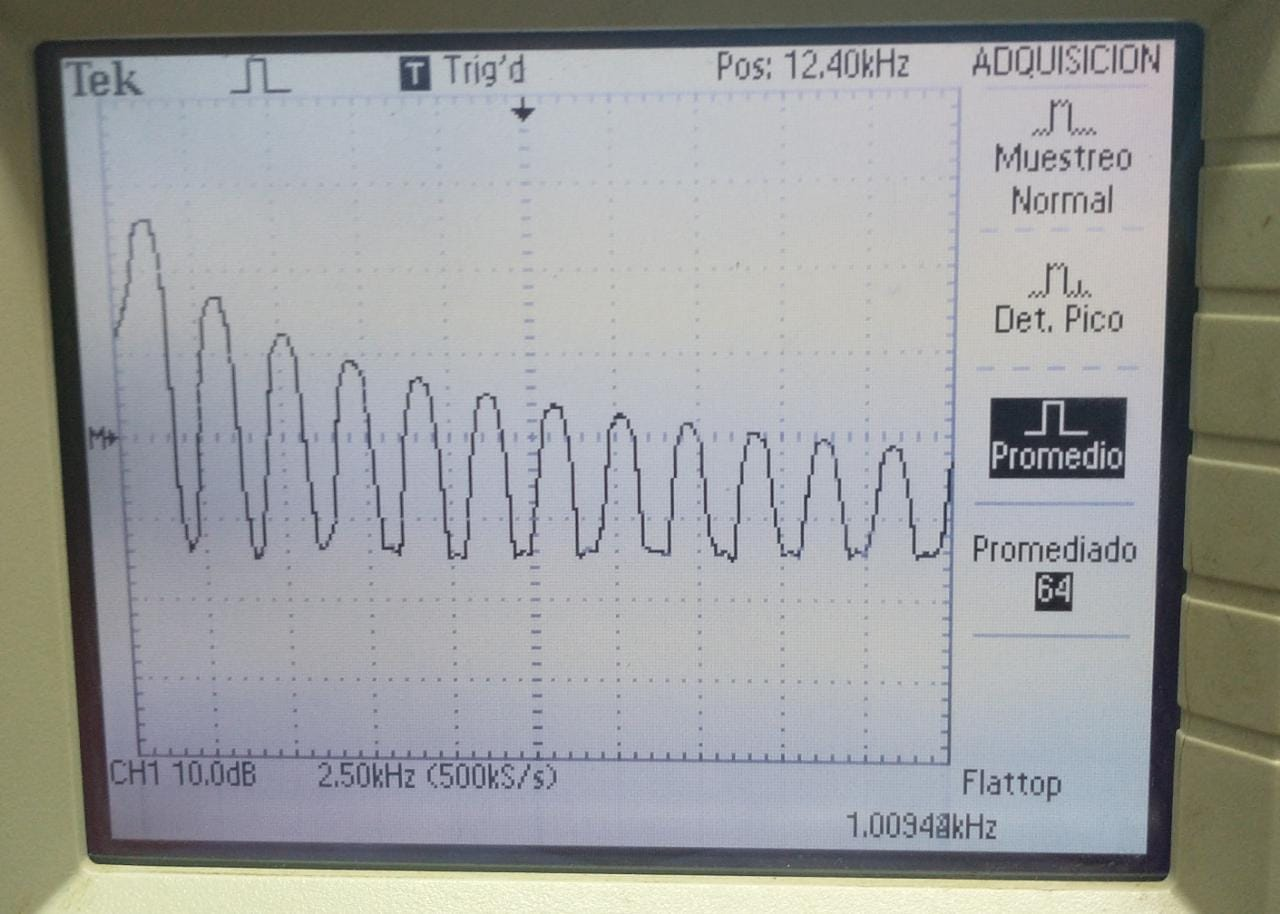
\includegraphics[width=\textwidth]{Imagenes/ActividadPractica/1AnalisisDeUnaSeñalCuadrada/Exp1_SeñalCuadrada_Promedio_Flattop.jpeg}}
        \caption{Con ventana Flattop.}
      \end{subfigure}
      \hfill 
      \begin{subfigure}[H]{0.40\textwidth}
        \frame{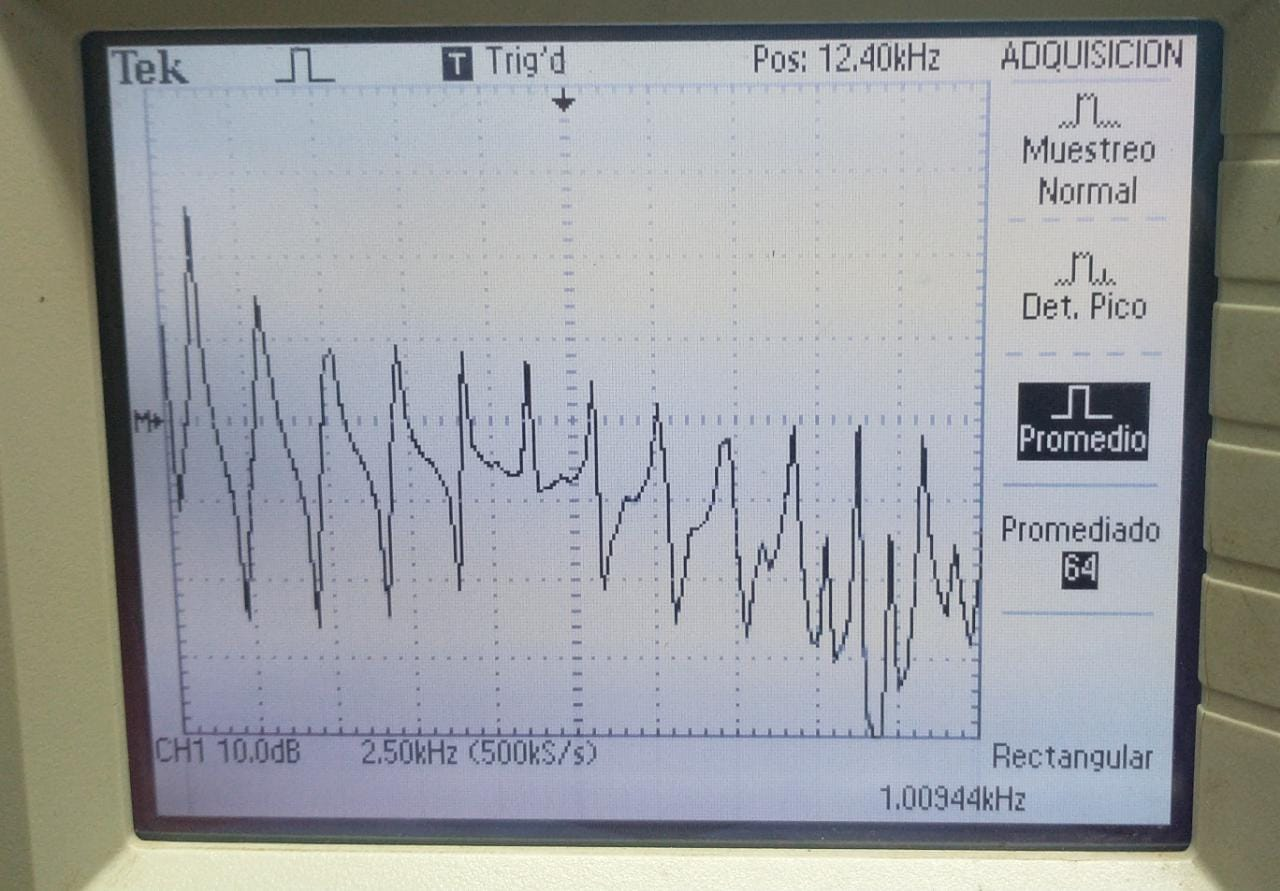
\includegraphics[width=\textwidth]{Imagenes/ActividadPractica/1AnalisisDeUnaSeñalCuadrada/Exp1_SeñalCuadrada_Promedio_Rectangular.jpeg}}
        \caption{Con ventana Rectangular.}
      \end{subfigure}
      \hfill 
      \begin{subfigure}[H]{0.40\textwidth}
        \frame{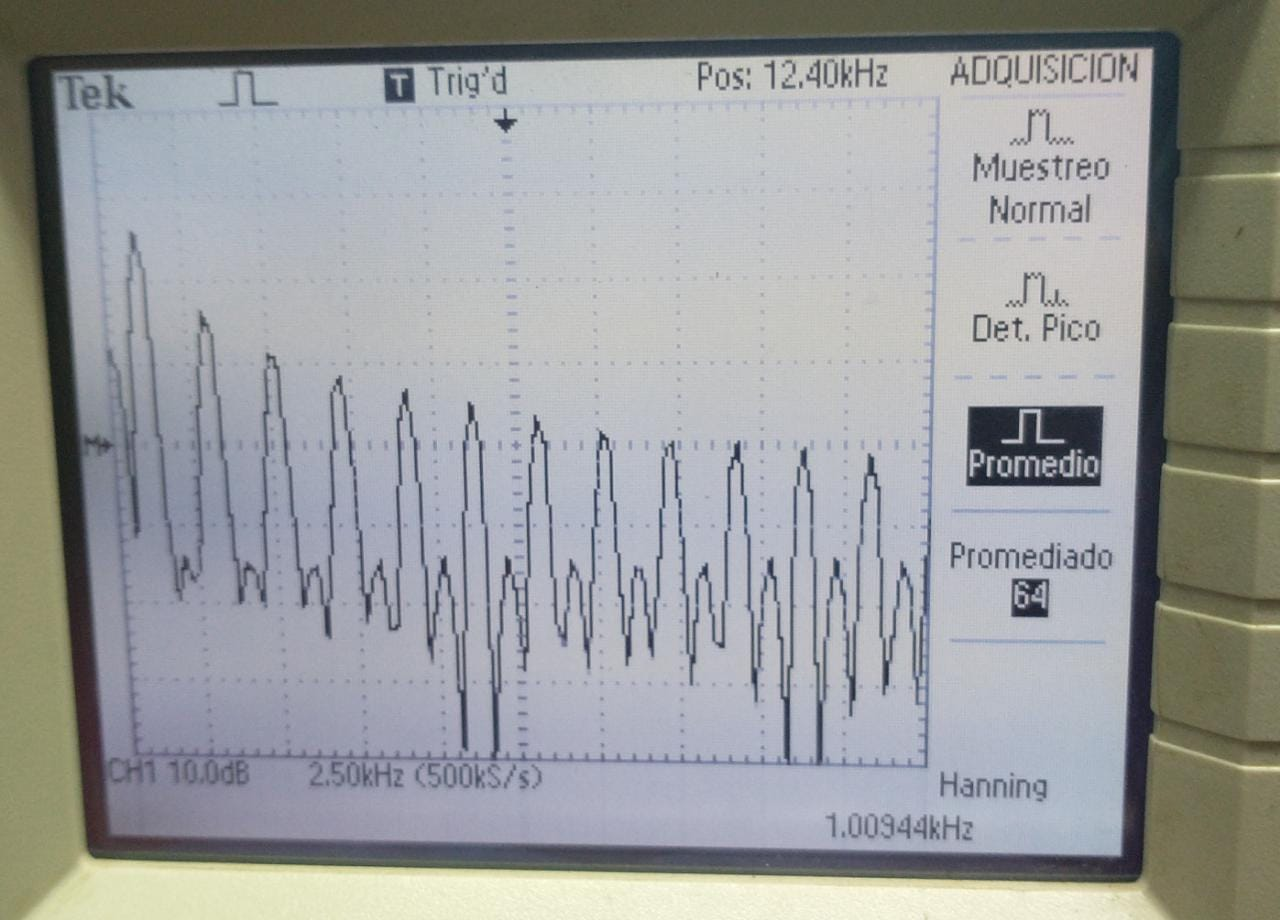
\includegraphics[width=\textwidth]{Imagenes/ActividadPractica/1AnalisisDeUnaSeñalCuadrada/Exp1_SeñalCuadrada_Promedio_Hanning.jpeg}}
        \caption{Con ventana de Hanning.}
      \end{subfigure}

      \caption{Señal cuadrada de $1~kHz$ con modo de adquisición de promedios.}
      \label{fig:SeñalCuadModoPromedio}
    \end{figure}

    
    \subsubsection{Medición de frecuencia}
      Para medir las \textbf{frecuencias} de los armónicos de la señal se hace uso de los cursores del osciloscopio.
      Además, se selecciona el modo de adquisición \textbf{Promedio} con 64 cuentas, y la ventana
      \textbf{Rectangular}. Los valores se encuentran en la Tabla~\ref{tab:ComponentesEspectrExp1}.

      \begin{table}[H]
        \centering
      \begin{tabular}{cccccccc} \hline \hline
        \textbf{Comp. Espectral}  &  \textbf{1}  &  \textbf{2}  & \textbf{3}  & \textbf{4} & \textbf{5}  & \textbf{6}  &  \textbf{7}\\ \hline
        \textbf{Frec. [kHz]}   &   $1,0$   &    $3,0$   &   $5,1$  &  $7,1$  &  $9,1$  &  $11,0$  &  $13,0$\\ \hline \hline
        \end{tabular}
        \caption{Frecuencias de las primeras 7 componentes espectrales.}
        \label{tab:ComponentesEspectrExp1}
      \end{table} 

      Las capturas con las mediciones de frecuencia realizadas con el osciloscopios encuentran en la 
      Figura~\ref{fig:SeñalCuad_MedicFrecOscilo}.

      \begin{figure}[H]
        \centering
        \begin{subfigure}[H]{0.40\textwidth}
          \frame{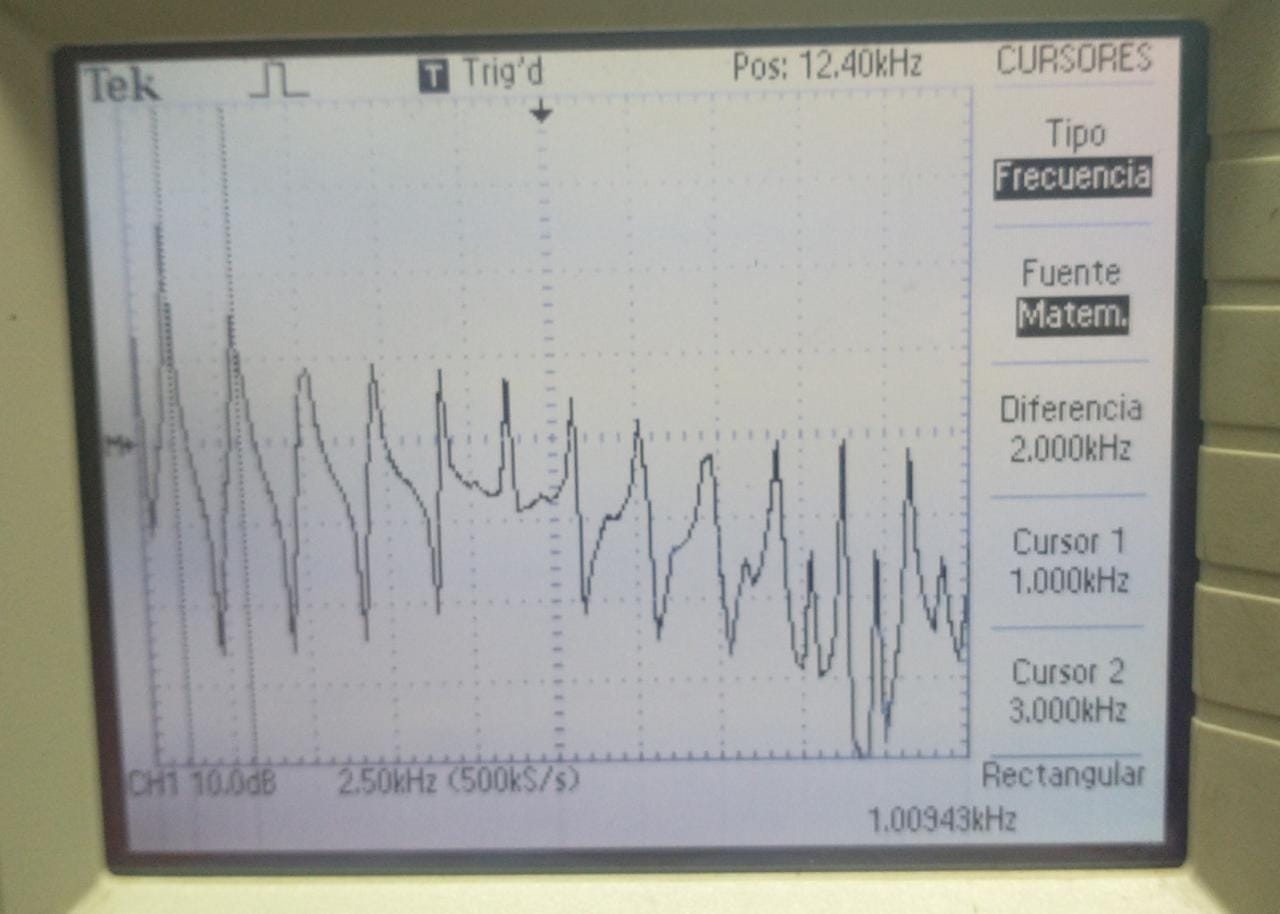
\includegraphics[width=\textwidth]{Imagenes/ActividadPractica/1AnalisisDeUnaSeñalCuadrada/Exp1_SeñalCuadrada_Frec_Armo1y2.jpeg}}
          \caption{Con ventana Flattop.}
        \end{subfigure}
        \hfill 
        \begin{subfigure}[H]{0.40\textwidth}
          \frame{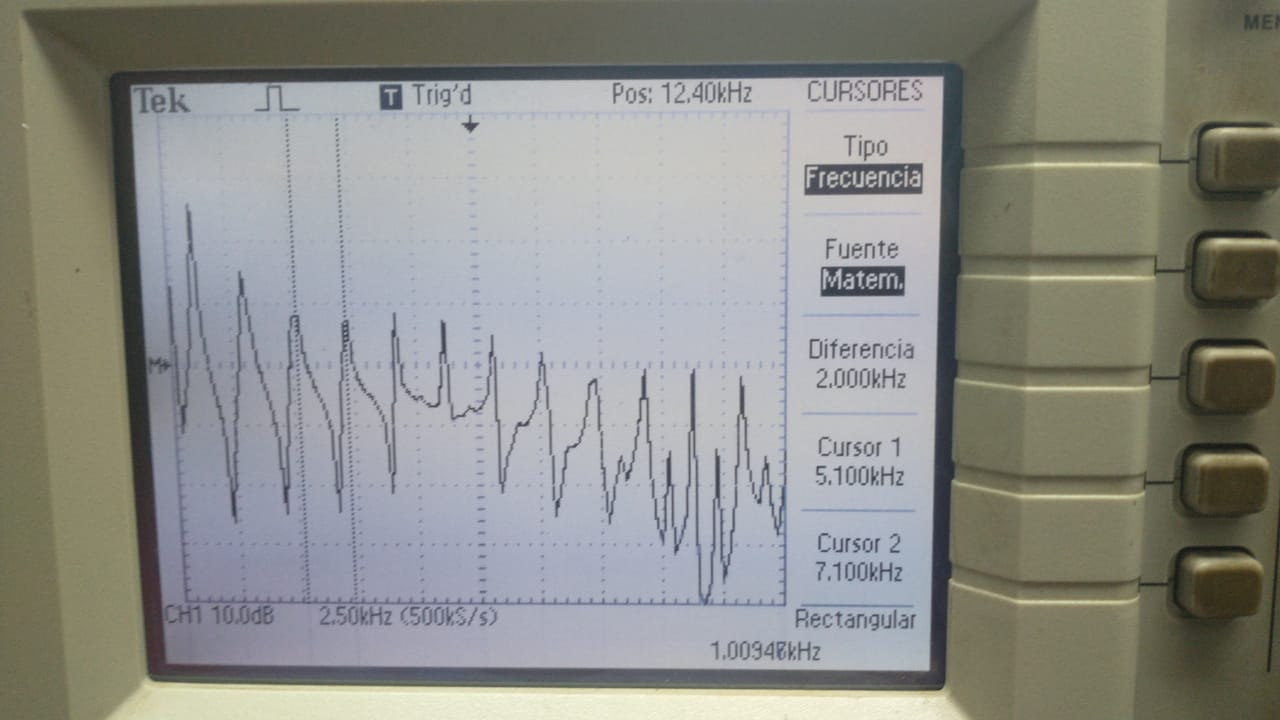
\includegraphics[width=\textwidth]{Imagenes/ActividadPractica/1AnalisisDeUnaSeñalCuadrada/Exp1_SeñalCuadrada_Frec_Armo3y4.jpeg}}
          \caption{Con ventana Rectangular.}
        \end{subfigure}
        \hfill 
        \begin{subfigure}[H]{0.40\textwidth}
          \frame{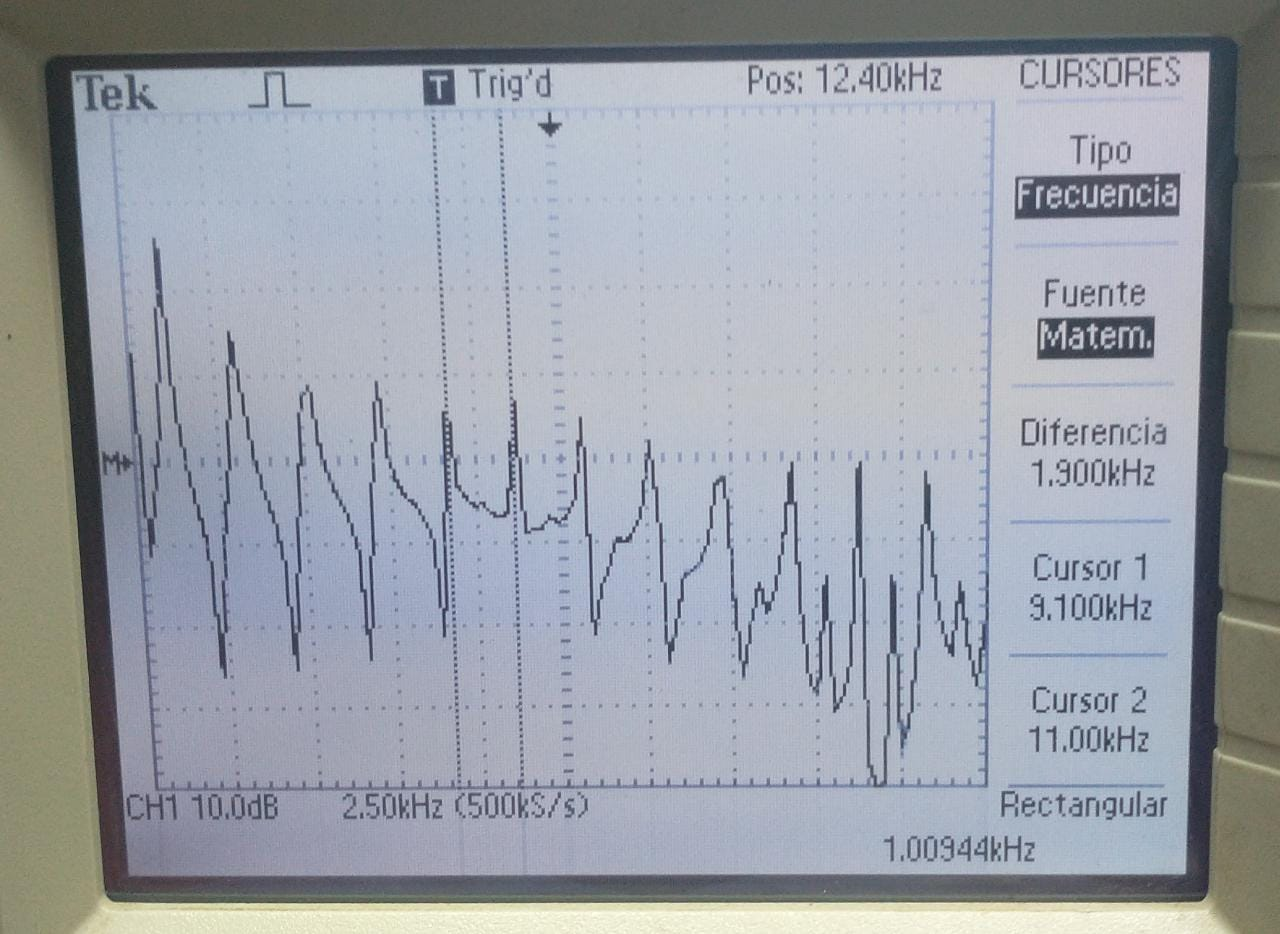
\includegraphics[width=\textwidth]{Imagenes/ActividadPractica/1AnalisisDeUnaSeñalCuadrada/Exp1_SeñalCuadrada_Frec_Armo5y6.jpeg}}
          \caption{Con ventana de Hanning.}
        \end{subfigure}
        \hfill 
        \begin{subfigure}[H]{0.40\textwidth}
          \frame{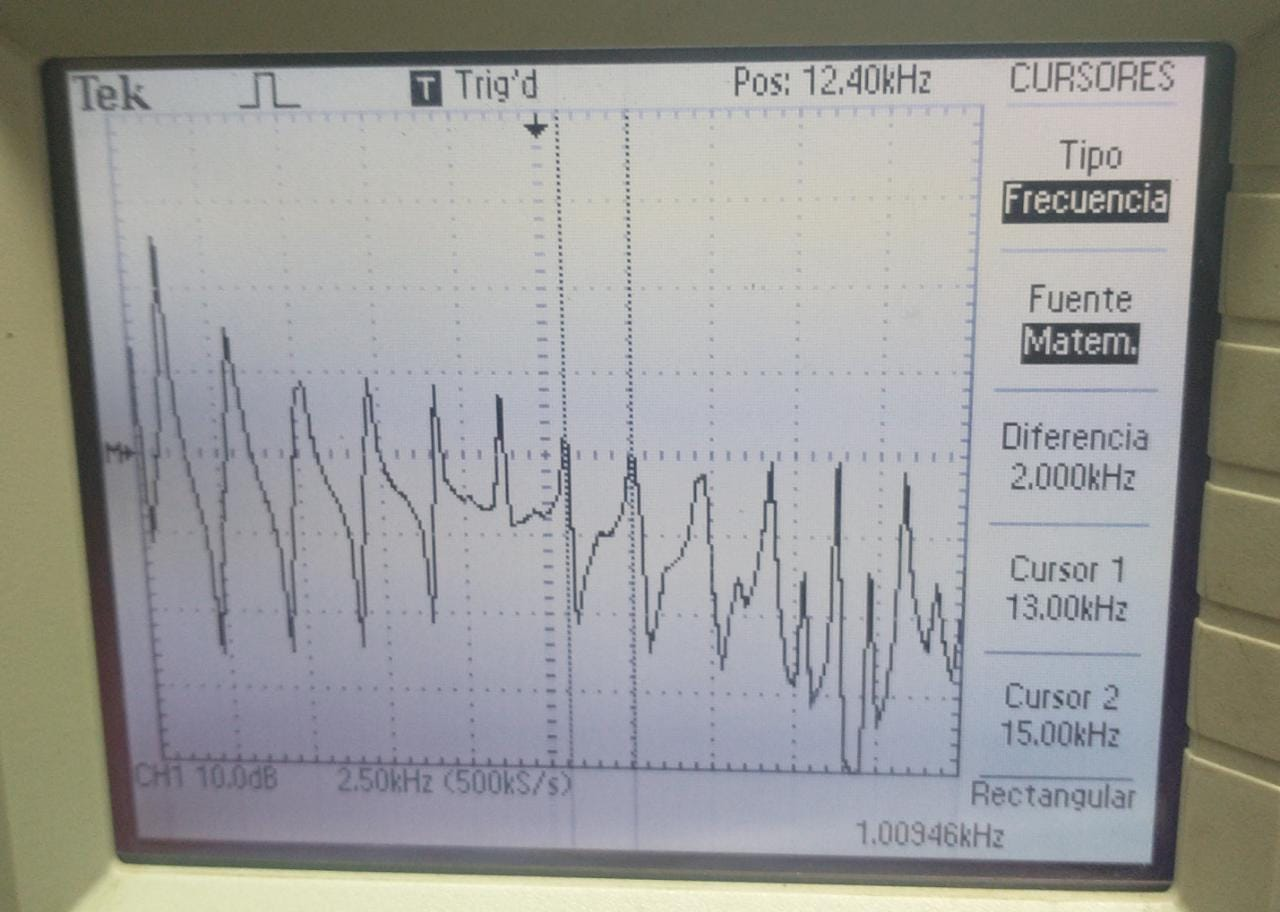
\includegraphics[width=\textwidth]{Imagenes/ActividadPractica/1AnalisisDeUnaSeñalCuadrada/Exp1_SeñalCuadrada_Frec_Armo7y8.jpeg}}
          \caption{Con ventana de Hanning.}
        \end{subfigure}

        \caption{Señal cuadrada de $1~kHz$ con modo de adquisición de promedios.}
        \label{fig:SeñalCuad_MedicFrecOscilo}
      \end{figure}

      
    \subsubsection{Medición de amplitud}
      Por último, se procede a medir la \textbf{amplitud} de las componentes espectrales de la señal. Para ello, se hace uso de los cursores
      del osciloscopio, previamente habiendo seleccionado la ventana \textbf{Flattop}. Vale aclarar que el osciloscopio realiza las mediciones
      en decibeles referenciados a 1~V (\textbf{dBv}). En la Tabla~\ref{tab:AmplitudEspectrExp1} se encuentran tabulados los resultados de la medición.

      \begin{table}[H]
        \centering
      \begin{tabular}{cccccccc} \hline \hline
        \textbf{Comp. Espectral}  &  \textbf{1}  &  \textbf{2}  & \textbf{3}  & \textbf{4} & \textbf{5}  & \textbf{6}  &  \textbf{7}\\ \hline
        \textbf{Tensión} &   $V_1$    &   $V_2$     &   $V_3$    &  $V_4$    &  $V_5$  &  $V_6$    &  $V_7$\\ \hline \hline
        $\mathbf{[dBv]}$ &   $-0,79$  &   $-10,2$   &   $-14,6$  &  $-17,8$  &  $-20$  &  $-21,4$  &  $-23,3$\\ \hline
        $\mathbf{[V]}$   &  $0,913$   &   $0,309$   & $0,186$    &  $0,129$  &  $0,1$  &  $0,085$  &  $0,068$ \\ \hline
        $\mathbf{[V^2]}$ &  $0,834$   &   $0,095$   & $0,035$    &  $0,016$  &  $0,01$ &  $0,007$  &  $0,005$ \\ \hline \hline
        \end{tabular}
        \caption{Amplitudes de las primeras 7 componentes espectrales.}
        \label{tab:AmplitudEspectrExp1}
      \end{table}

      Partiendo del Teorema de Parseval, se puede obtener el valor eficaz de la señal mediante la amplitud de sus componentes espectrales

      \begin{align*}
                        V_{RMS} &= \sqrt{V_1^2 + V_2^2 + V_3^2 + V_4^2 + V_5^2 + V_6^2 + V_7^2}  \\
        \Longrightarrow V_{RMS} &= \sqrt{0,834 + 0,095 + 0,035 + 0,016 + 0,01 + 0,007 + 0,005 } \\
      \end{align*}

      \vspace{-25pt}
      $$\therefore \hspace{20pt} \boxed{V_{RMS}=1,00~[V]}$$

      Las capturas de las mediciones realizadas de las primeras cuatro componentes armónicas
      se encuentran en la Figura~\ref{fig:SeñalCuad_MedicAmplOscilo}.

      \begin{figure}[H]
        \centering
        \begin{subfigure}[H]{0.40\textwidth}
          \frame{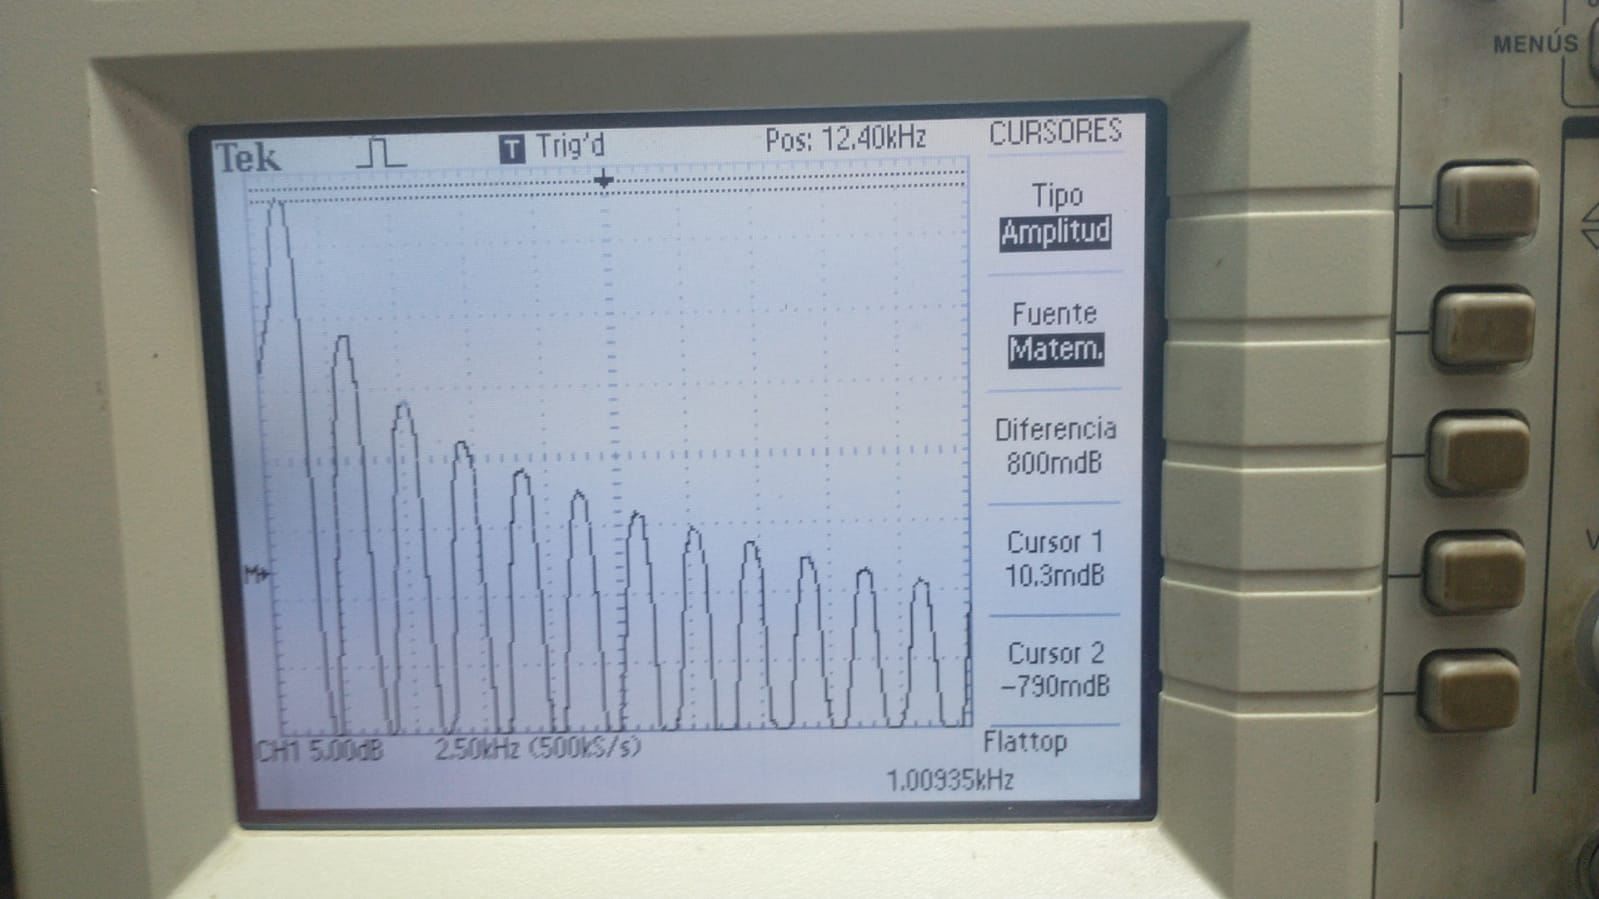
\includegraphics[width=\textwidth]{Imagenes/ActividadPractica/1AnalisisDeUnaSeñalCuadrada/Exp1_SeñalCuadrada_Ampl_Armo1.jpeg}}
          \caption{1er armónico.}
        \end{subfigure}
        \hfill 
        \begin{subfigure}[H]{0.40\textwidth}
          \frame{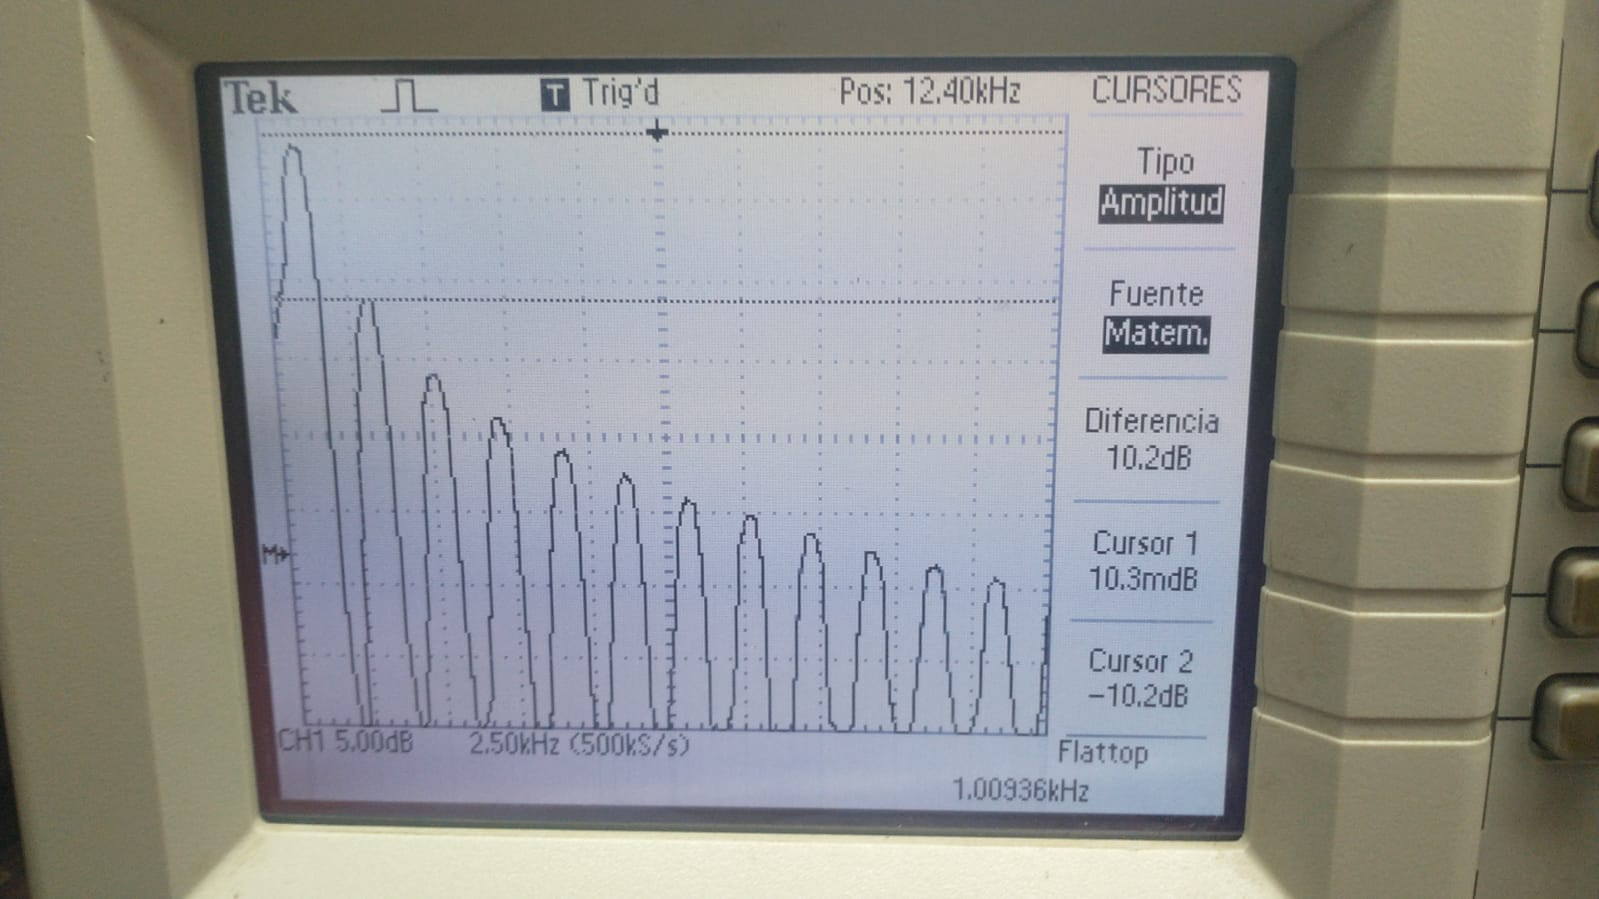
\includegraphics[width=\textwidth]{Imagenes/ActividadPractica/1AnalisisDeUnaSeñalCuadrada/Exp1_SeñalCuadrada_Ampl_Armo2.jpeg}}
          \caption{2do armónico.}
        \end{subfigure}
        \hfill 
        \begin{subfigure}[H]{0.40\textwidth}
          \frame{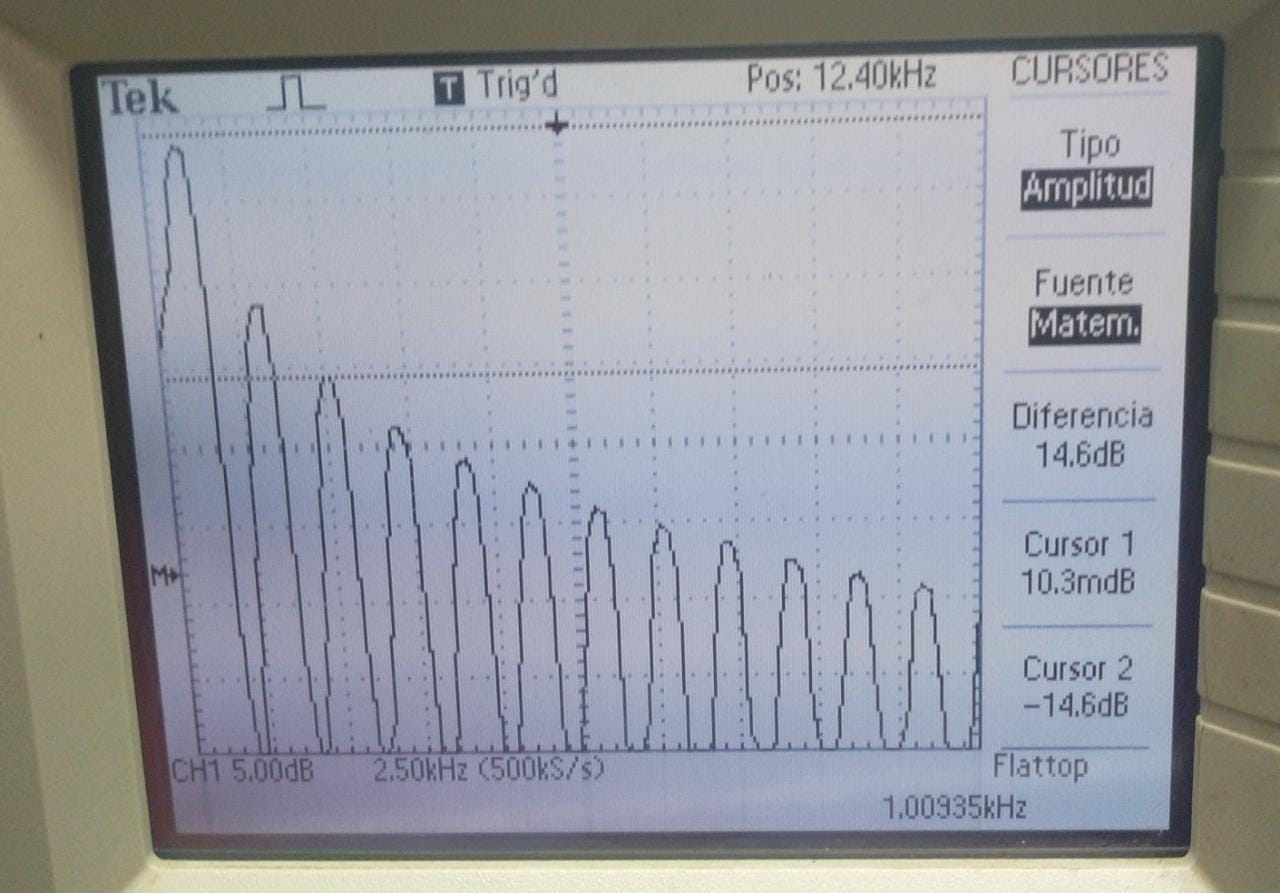
\includegraphics[width=\textwidth]{Imagenes/ActividadPractica/1AnalisisDeUnaSeñalCuadrada/Exp1_SeñalCuadrada_Ampl_Armo3.jpeg}}
          \caption{3er armónico.}
        \end{subfigure}
        \hfill 
        \begin{subfigure}[H]{0.40\textwidth}
          \frame{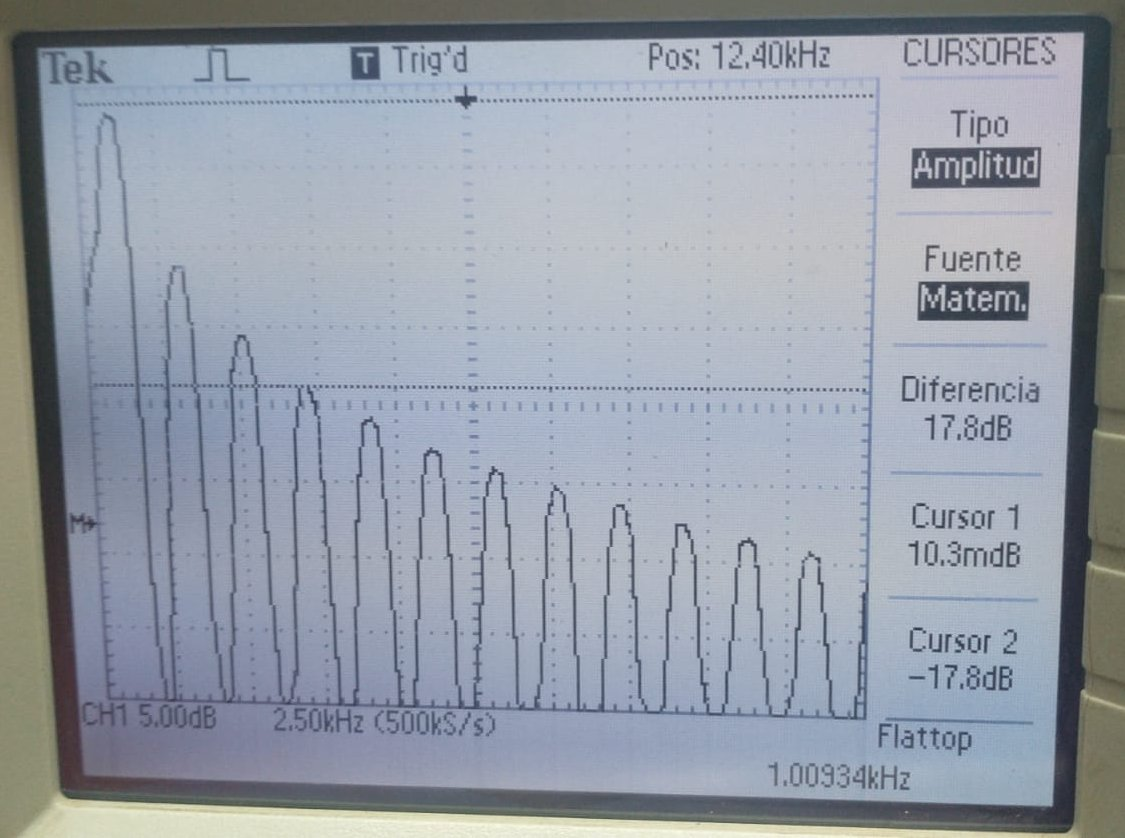
\includegraphics[width=\textwidth]{Imagenes/ActividadPractica/1AnalisisDeUnaSeñalCuadrada/Exp1_SeñalCuadrada_Ampl_Armo4.jpeg}}
          \caption{4to armónico.}
        \end{subfigure}

        \caption{Amplitudes de las primeras 4 componentes espectrales de la señal.}
        \label{fig:SeñalCuad_MedicAmplOscilo}
      \end{figure}

      Como corroboración, se hace uso de la herramienta del osciloscopio que permite medir el
      valor eficaz de una señal en el tiempo. El valor coincide con el calculado mediante 
      las componentes espectrales - véase Figura~\ref{fig:CorroboraVrms}.

      \begin{figure}[H]
        \centering
        \frame{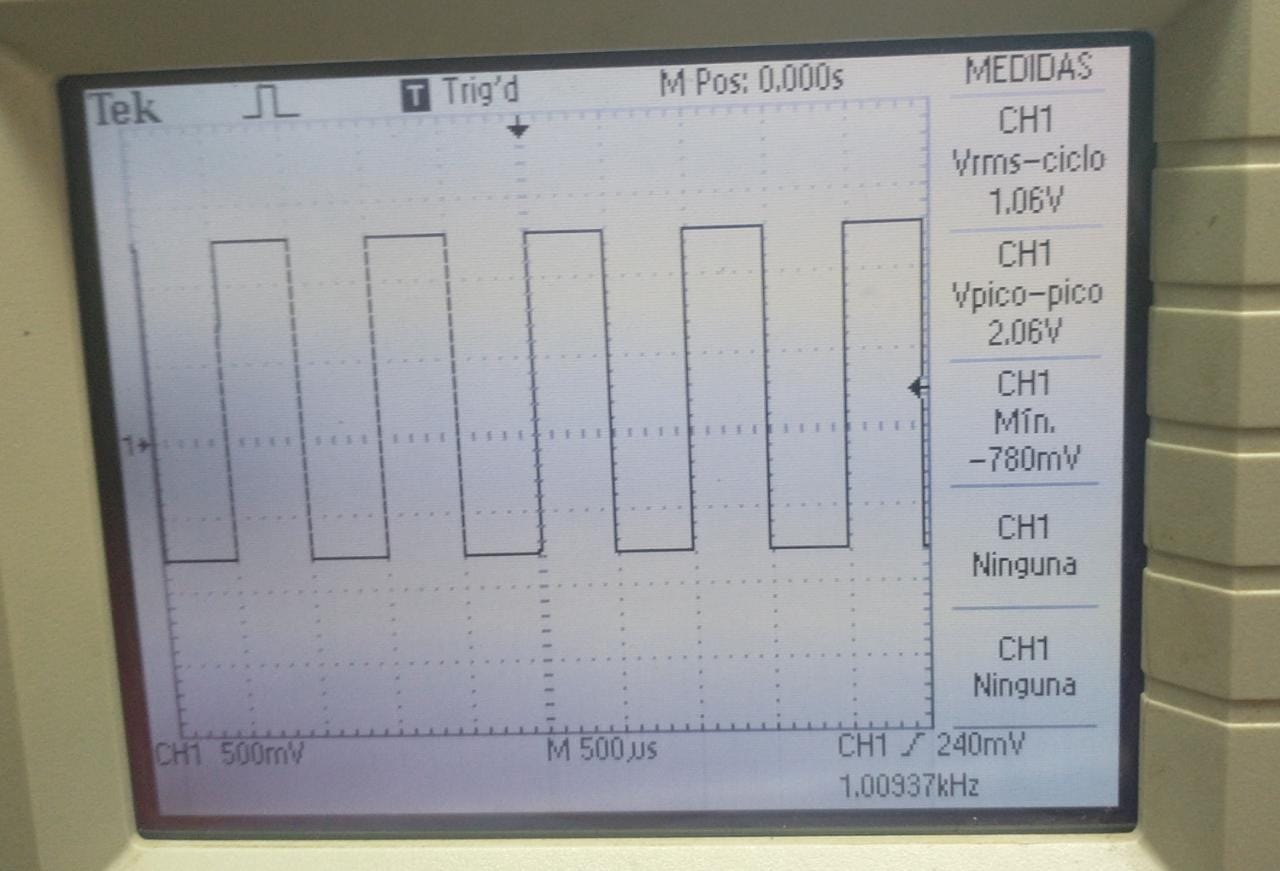
\includegraphics[width=0.4\textwidth]{Imagenes/ActividadPractica/1AnalisisDeUnaSeñalCuadrada/Exp1_SeñalCuadrada_CorroboracionVrms.jpeg}}
        \caption{Corroboración del valor de tensión eficaz de la señal.}
        \label{fig:CorroboraVrms}
      \end{figure}


    \pagebreak
